\documentclass{article}
\usepackage{amsmath} 
\usepackage{graphicx} 
\usepackage{authblk}
\usepackage{url}
\usepackage{multirow}

\title{Application and Comparison of Different Numerical Methods for One-dimensional Poisson's Equation}
\author[1]{Tong Li}
\affil[1]{Department of Physics and Astronomy, Michigan State University}
\date{}

\begin{document}
	\maketitle
	\begin{abstract}
	Poisson's equation is an important type of differential equations in science and engineering, 
	and thus it is valuable to study numerical methods for it.  
	In this report we numerically solve a one-dimensional Poisson's equation (with Dirichlet boundary conditions)
	on an equidistant grid 
	by converting it into a set of linear equations $\mathbf{A}\mathbf{v}=\mathbf{\overline{f}}$ 
	where $\mathbf{A}$ is a tri-diagonal matrix. 
	Three numerical methods are discussed and compared in this report: 
	Gaussian elimination for a general tri-diagonal matrix (M1), 
	a special method that makes use of the fact that matrix $\mathbf{A}$ has identical elements along the diagonal and identical (but different) values for the non-diagonal elements (M2), 
	and LU decomposition (M3). 
	The relative errors of these methods are consistent with the approximation error introduced in discretization, 
	and M2 is the most efficient algorithm as it uses the property of this problem to do precalculation. 
	\end{abstract}

	\section{Introduction}
	Poisson's equation is one important type of differential equations in science and engineering, 
	especially in electromagnetism. 
	Poisson's equation has the following form: 
	\begin{equation}
	\nabla^{2} u\left( \vec{r}\right)  = f\left( \vec{r} \right) \ ,
	\end{equation}
	where $f\left( \vec{r}\right)$ is known and 
	$u\left( \vec{r}\right)$ is the function to be solved. 
	In electrostatics, $u\left( \vec{r}\right)$ is the electric potential and 
	$f\left( \vec{r}\right)=-4\pi \rho\left( \vec{r} \right)$ 
	where $\rho\left( \vec{r} \right) $ is charge density. 
	In physics, Poisson's equation usually comes with different kinds of boundary value conditions, 
	such as Dirichlet (values of $u\left( \vec{r}\right)$ are specified on boundaries), 
	or Neumann (normal derivatives $\frac{\partial u}{\partial n}$ are specified on boundaries) 
	boundary conditions. 
	\par
	Poisson's equation can be analytically solved by separation of variables and eigenfunction method, 
	which usually gives $u\left( \vec{r}\right)$ as an infinite series. 
	However, when the inhomogeneous term $f(x)$ or boundary conditions become very complicated, 
	it is impossible to find an analytical solution. 
	Therefore, it is important to study the numerical methods to solve Poisson's equations. 
	\par
	For simplicity, we will focus on one-dimensional Poisson's equation 
	with Dirichlet boundary conditions in this report. 
    In section \ref{method} we will describe the three numerical methods 
    used to solve the Poisson's equation. 
    Section \ref{result} will discuss the numerical error and speed of these methods. 
    Conclusions and perspective will be given in section \ref{conclude}. 
	
	\section{Numerical methods}\label{method}
	The one-dimentional Poisson's equation can be written as
	\begin{equation}\label{diff}
	-u''(x) = f(x)\ .
	\end{equation}
	This equation will be solved in the region $x \in [0,1]$, 
	with boundary condition $u(0)=u(1)=0$. 
	\par
	First, the discretized approximation to function $u$ is defined as $v_i$ 
	on $(n+1)$ equidistant points $x_i \in [0,1]$, 
	where $x_0=0$ and $x_n=1$. Thus, the step length is $h=1/n$ and $x_i=ih$. 
	\par
	By Taylor expansion, we have
	\begin{eqnarray}
	u(x+h)&=&u(x)+u'(x)h+\frac{1}{2}u''(x)h^2+O(h^2)\ ,
	\\
	u(x-h)&=&u(x)-u'(x)h+\frac{1}{2}u''(x)h^2+O(h^2)\ .
	\end{eqnarray}
	By adding the two equations above, we can approximate the second derivative as
	\begin{equation}\label{diffappr}
	u''(x_i)=\frac{v_{i+1}+v_{i-1}-2v_i}{h^2}+O(h^2)
	\end{equation}
	where the approximation error is $O(h^2)$. 
	\par
	So the problem can be converted to a set of linear equations
	\begin{equation}
	-\frac{v_{i+1}+v_{i-1}-2v_i}{h^2} = f_i  \hspace{0.5cm} \mathrm{for} \hspace{0.1cm} i=1,2, \dots, n-1
	\end{equation}
	where $f_i=f(x_i)$. 
	This set of equations can be rewritten as 
	\begin{equation}\label{mateq}
	\mathbf{A}\mathbf{v} = \overline{\mathbf{f}}\ ,
	\end{equation}
	where $\mathbf{A}$ is a $(n-1) \times (n-1)$  tridiagonal matrix 
	\begin{equation}\label{matA}
	\mathbf{A} = \begin{bmatrix}
	2& -1& 0 &\dots   & \dots &0 \\
	-1 & 2 & -1 &0 &\dots &\dots \\
	0&-1 &2 & -1 & 0 & \dots \\
	& \dots   & \dots &\dots   &\dots & \dots \\
	0&\dots   &  &-1 &2& -1 \\
	0&\dots    &  & 0  &-1 & 2 \\
	\end{bmatrix}
	\end{equation}
	and $\overline{f}_i=h^2f_i$.
	Now we will discuss the three numerical methods to solve Eq. \ref{mateq}. 
	\subsection{Gaussian elimination for a general tri-diagonal matrix}\label{m1}
	In this subsection we will solve $\mathbf{A}\mathbf{v} = \overline{\mathbf{f}}$
	for any tri-diagonal matrix $\mathbf{A}$ using Gaussian elimination. 
	The equation is written as 
	\begin{equation}\label{gentri}
	\mathbf{A}\mathbf{u} = \begin{bmatrix}
	b_1& c_1& 0 &\dots   & \dots &0 \\
	a_2 & b_2 & c_2 &0 &\dots &\dots \\
	0&a_3 &b_3 & c_3 & 0 & \dots \\
	& \dots   & \dots &\dots   &\dots & \dots \\
	0&\dots   &  &a_{n-2} &b_{n-2}& c_{n-2} \\
	0&\dots    &  & 0  &b_{n-1} & c_{n-1} \\
	\end{bmatrix}
	\begin{bmatrix}
	u_1 \\
	u_2 \\
	u_3 \\
	\dots \\
	u_{n-2} \\
	u_{n-1}
	\end{bmatrix}
	=
	\begin{bmatrix}
	\overline{f}_1 \\
	\overline{f}_2 \\
	\overline{f}_3 \\
	\dots \\
	\overline{f}_{n-2} \\
	\overline{f}_{n-1}
	\end{bmatrix}
	=\overline{\mathbf{f}}\ .
	\end{equation}
	In the $i$-th step of Gaussian elimination, the product of $-\frac{a_i}{\tilde{b}_{i-1}}$ 
	(where $\tilde{b}_{i-1}$ is the new diagonal element obtained in the previous step) and row $i$
	is added to row $(i+1)$, giving a new diagonal element
	\begin{equation}\label{tildeb}
	\tilde{b_{i}}=b_i-\frac{a_i c_{i-1}}{\tilde{b}_{i-1}}\quad i=2,3,\dots,n-1
	\end{equation}
	and a new right-hand side 
	\begin{equation}\label{tildef}
	\tilde{f}_i=\overline{f}_i-\frac{a_i \tilde{f}_{i-1}}{\tilde{b}_{i-1}}\quad i=2,3,\dots,n-1\ . 
	\end{equation}
	And we always have $\tilde{b}_1=b_1$ and $\tilde{f}_1=\overline{f}_1$. 
	Then the equation becomes 
	\begin{equation}
	\tilde{\mathbf{A}}\mathbf{u} = \begin{bmatrix}
	\tilde{b}_1& c_1& 0 &\dots   & \dots &0 \\
	0 & \tilde{b}_2 & c_2 &0 &\dots &\dots \\
	0&0 &\tilde{b}_3 & c_3 & 0 & \dots \\
	& \dots   & \dots &\dots   &\dots & \dots \\
	0&\dots   &  &0 &\tilde{b}_{n-2}& c_{n-2} \\
	0&\dots    &  & 0  &\tilde{b}_{n-1} & c_{n-1} \\
	\end{bmatrix}
	\begin{bmatrix}
	u_1 \\
	u_2 \\
	u_3 \\
	\dots \\
	u_{n-2} \\
	u_{n-1}
	\end{bmatrix}
	=
	\begin{bmatrix}
	\tilde{f}_1 \\
	\tilde{f}_2 \\
	\tilde{f}_3 \\
	\dots \\
	\tilde{f}_{n-2} \\
	\tilde{f}_{n-1}
	\end{bmatrix}
	=\tilde{\mathbf{f}}
	\end{equation}
	which can be solved by backward substitution 
	\begin{eqnarray}\label{backward}
	\nonumber
	u_{n-1}&=&\frac{\tilde{f}_{n-1}}{\tilde{b}_{n-1}} \\
	u_{i}&=&\frac{\tilde{f}_i-c_i u_{i+1}}{\tilde{b}_i}\quad i=n-2,n-3,\dots,1\ .
	\end{eqnarray}
	This algorithm needs $[8(n-2)+1]$ floating-point operations (FLOPs), and 
	its time complexity is $O(n)$. 
	
	\subsection{A special method for this problem}\label{m2}
	By Eq. \ref{matA} and \ref{gentri}, we can see that $a_i=c_i=-1$ and $b_i=2$ for any $i$.  
	Thus, Eq. \ref{tildeb} becomes 
	\begin{equation}
	\tilde{b}_i=2-\frac{1}{\tilde{b}_{i-1}}
	\end{equation}
	which yields  
	\begin{equation}\label{spetildeb}
	\tilde{b}_i=\frac{i+1}{i}\ . 
	\end{equation}
	Therefore, $\tilde{\mathbf{b}}$ can be calculated beforehand, 
	which eliminates redundant calculations when we change function $f(x)$.
	\par 
	Eq. \ref{tildef} and \ref{spetildeb} yield 
	\begin{equation}
	\tilde{f}_i=\overline{f}_i+\frac{(i-1)\tilde{f}_{i-1}}{i}\ .
	\end{equation}
	and then the backward substitution (Eq. \ref{backward}) can be written as
	\begin{eqnarray}
	\nonumber
	u_{n-1}&=&\frac{n-1}{n}\tilde{f}_{n-1} \\
	u_{i}&=&\frac{i}{i+1}\left(\tilde{f}_{i}+u_{i+1}\right)\quad i=n-2,n-3,\dots,1\ .
	\end{eqnarray}
	Since $\tilde{\mathbf{b}}$ can be precalcuated, 
	we do not consider Eq. \ref{spetildeb} when counting FLOPs. 
	So this algorithm needs $[4(n-2)+1]$ FLOPs, 
	and its time complexity is also $O(n)$. 
	
	
	\subsection{LU decomposition}\label{m3}
	For a general (not necessarily tri-diagonal) matrix $\mathbf{A}$, 
	equation $\mathbf{A}\mathbf{v} = \overline{\mathbf{f}}$	is usually solved by LU decomposition. 
	First, matrix $\mathbf{A}$ is decomposed as $\mathbf{A}=\mathbf{L}\mathbf{U}$, 
	where $\mathbf{L}$ and $\mathbf{U}$ are upper- and lower-triangular matrices, respectively. 
	Then the equation $\mathbf{A}\mathbf{v} = \overline{\mathbf{f}}$ becomes 
	\begin{eqnarray}
	\mathbf{L}\mathbf{w} &=& \overline{\mathbf{f}} \label{loweq}
	\\
	\mathbf{U}\mathbf{v} &=& \mathbf{w} \label{upeq}
	\end{eqnarray}
	Eq. \ref{loweq} and \ref{upeq} can be easily solved by forward and backward substitution, respectively. 
	The time complexity of LU decomposition is $O(n^3)$, 
	which is much larger than the methods discussed in section \ref{m1} and \ref{m2}.
	In this work we use the LU decomposition algorithm in Armadillo (a C++ linear algebra library). 
	
	\section{Results and discussion}\label{result}
	In this section we will discuss the results of the three numerical methods described in section \ref{method}. 
	The three methods discussed in section \ref{m1}, \ref{m2} and \ref{m3} are denoted as M1, M2 and M3, respectively.  
	For benchmark, we choose $f(x)=100 e^{-10x}$, which gives an analytical
	solution of Eq. \ref{diff}: 
	\begin{equation}
	u(x)=1-\left(1-e^{-10}\right)x-e^{-10x}\ .
	\end{equation}
	The relative error at point $x_i$ is defined as 
	\begin{equation}
	\epsilon_i=\left| \frac{v_i-u(x_i)}{u(x_i)}\right|\ .
	\end{equation}
	\par
	\begin{figure}[tb]
		\centering
		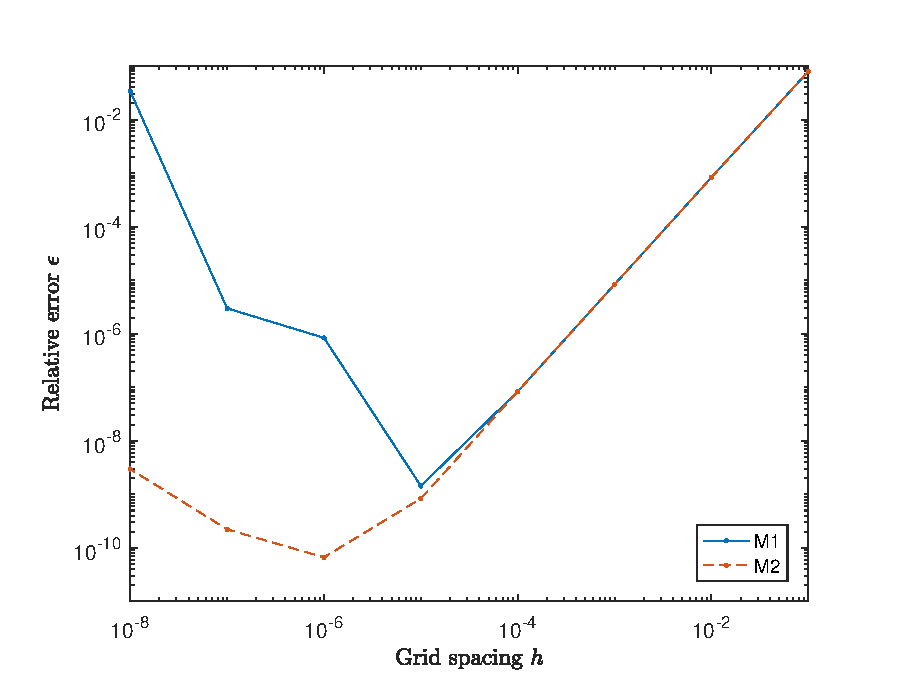
\includegraphics[width=\textwidth]{fig_error.eps}
		\caption{Maximum relative errors of M1 and M2 for different grid spacing $h$. }
		\label{fig:error}
	\end{figure}
	The maximum relative errors of methods M1 and M2 for different grid spacing $h$ are shown in Figure \ref{fig:error}. 
	These errors are small enough to confirm the correctness of our program. 
	In the region of $h=10^{-1} \sim 10^{-4}$, M1 and M2 have the same relative errors $\epsilon$. 
	The logarithm of $\epsilon$ decreases linearly as $\log h$ decreases, with a slope of 2. 
	So in this region the relative error is $O(h^2)$, the same as the approximation error given in Eq. \ref{diffappr}. 
	When $h<10^{-4}$, the relative error begins to fall down slowly and even increase as $h$ decreases, 
	which indicates that the round-off error becomes important for very small $h$. 
	In Eq. \ref{diffappr}, both $(v_{i+1}-v_i)$ and $(v_{i-1}-v_i)$ give an $\epsilon_M=O(10^{-15})$ 
	round-off error (for double precision), 
	and thus the round-off error should be $O(\frac{10^{-15}}{h^2})$ for $u''(x_i)$. 
	Therefore, when $h=10^{-4}\sim 10^{-5}$, $O(\frac{10^{-15}}{h^2})\approx O(h^2)$, i.e. 
	the round-off and approximation error become comparable. 
	So we should not use grid spacing $h<10^{-4}$ when the round-off error contribute significantly to our loss of precision. 
	\par
	Because of memory and time limitation, M3 cannot go to $h<10^{-3}$. 
	For $h\geq 10^{-3}$, M3 gives the same relative errors as M1 and M2, which are not shown in Figure \ref{fig:error}. 
	\par
	\begin{table}[tb]
		\centering
		\caption{Time used by M1 and M2 for different number of grid points $n$. 
		Each value given in this table is the average over three measurements. 
	    For M2 the time of precalculating Eq. \ref{spetildeb} is not included. }
		\begin{tabular}{cccc}
			\hline
			\hline
			\multirow{2}{*}{$n$} &\multirow{2}{*}{$h$}& \multicolumn{2}{c}{Time (sec)}\\
			& & M1 & M2  \\
			\hline
			$10^6$&$10^{-6}$&0.0469 & 0.0313 \\
			$10^7$&$10^{-7}$&0.3698 & 0.1875\\
			$10^8$&$10^{-8}$&7.0729 & 2.4323\\
			\hline
			\hline
		\end{tabular}
		\label{table:time}
	\end{table}
	Table \ref{table:time} shows the time used by algorithms M1 and M2 for different number of grid points $n$, 
	with no optimization flag applied. 
	In order to measure the time accurately, $n$ is chosen to be large enough ($10^6,\ 10^7\text{ and }10^8$), 
	and each value given in Table \ref{table:time} is the average over three measurements. 
	For M2, the time of precalculating Eq. \ref{spetildeb} is not included. 
	As $n$ increases, the time of both M1 and M2 rises almost linearly, corresponding to their O(n) time complexity. 
	In addition, M2 is much faster than M1 because Eq. \ref{spetildeb} is precalculated in M2. 
	For the same $n$, M2's FLOPs is about half of M1's, and the time of M2 is also roughly half of M1's. 
	Therefore, from the perspective of efficiency, 
	M2 is the best option to solve a one-dimensional Poisson's equation with Dirichlet boundary conditions, 
	especially when we want to change the inhomogeneous term $f(x)$ many times. 
	
	\section{Conclusions and outlook}\label{conclude}
	In this report we discuss three numerical methods to solve a one-dimensional Poisson's equation 
	with Dirichlet boundary conditions. 
	First, this problem is discretized on equidistant grid points with spacing $h$, and converted into a set of linear equations 
	$\mathbf{A}\mathbf{v} = \overline{\mathbf{f}}$ where $\mathbf{A}$ is a tri-diagonal matrix. 
	Then we describe three numerical methods to solve this equation: 
	Gaussian elimination for a general tri-diagonal matrix (M1, section \ref{m1}), 
	a special method that makes use of the fact that matrix $\mathbf{A}$ has identical elements along the diagonal and identical (but different) values for the non-diagonal elements (M2, section \ref{m2}), 
	and LU decomposition (M3, section \ref{m3}). 
	\par
	In section \ref{result} we apply the three methods to solve $-u''(x)=100 e^{-10x}$ whose analytical solution is known. 
	The small relative errors extracted from our program confirm the correctness of these algorithms. 
	When $h=10^{-1} \sim 10^{-4}$ the relative error $\epsilon \sim h^2$, which is consistent with the approximation error
	of the second derivative (Eq. \ref{diffappr}). When $h<10^{-4}$ round-off error becomes more and more dominant as $h$ decreases. 
	Thus the optimal grid spacing $h$ is $10^{-4}$. 
	Comparing the time used by these methods, we find that M2 is the most efficient one 
	because it fully utilizes the property of this problem to precalculate. 
	The advantage of M2 will be more significant if we want to change the inhomogeneous term many times. 
	\par
	Although the Poisson's equation we usually see is two- or three-dimensional, 
	the algorithms for one-dimensional Poisson's equation are still useful because
	many high-dimensional problems can be reduced to one dimension by methods like separation of variables. 
	In addition, this project provides numerical algorithms to solve linear equation $\mathbf{A}\mathbf{x}=\mathbf{b}$ 
	where $\mathbf{A}$ is a tri-diagonal matrix. 
	This type of problem often appears in science and engineering, so it is important to understand
	all the numerical methods discussed in this report. 
	
	\section*{Acknowledgments}
	I am grateful for the sincere guidance from Prof. Morten Hjorth-Jensen, and
	I also want to thank Mengzhi Chen for helpful discussions. 
	
	\nocite{*} 
	\bibliographystyle{plain}
	\bibliography{proj1_ref}
\end{document}